\chapter{Despliegue de la aplicación}
En la etapa de despliegue es cuando el software queda disponible para el uso y disfrute de
los usuarios. Supone una etapa fundamental para dar por finalizada la construcción del
software. 

Necesito que el modelo de computación en la nube me provea de facilidad suficiente para
añadir y desplegar nueva funcionalidad con rapidez. El coste tiene que ser lo más
inteligente y adaptado posible. Y además, quiero un sistema que me prevea de una
plataforma ya estructurada de forma que solo tenga que centrarme en la configuración
correcta de mi servidor de acorde con los requisitos de la plataforma sin tener que
configurar ninguna infraestructura de bajo nivel ni tan siquiera el sistema operativo.

Estos requisitos hacen utilizar un entorno cloud un PaaS, \textit{Platform as a service}
donde tendré varias capas de servicios apilados lo que me va a permitir ejecutar y
gestionar mis aplicación desplegada sin tener que mantener la infraestructura subyacente.

A la hora de elegir un modelo de entorno cloud tenemos distintos modelos de cloud
computing, dependiendo de las partes de la infraestructura local que queramos gestionar.

\FloatBarrier
\begin{figure}[h]
	\centering	
	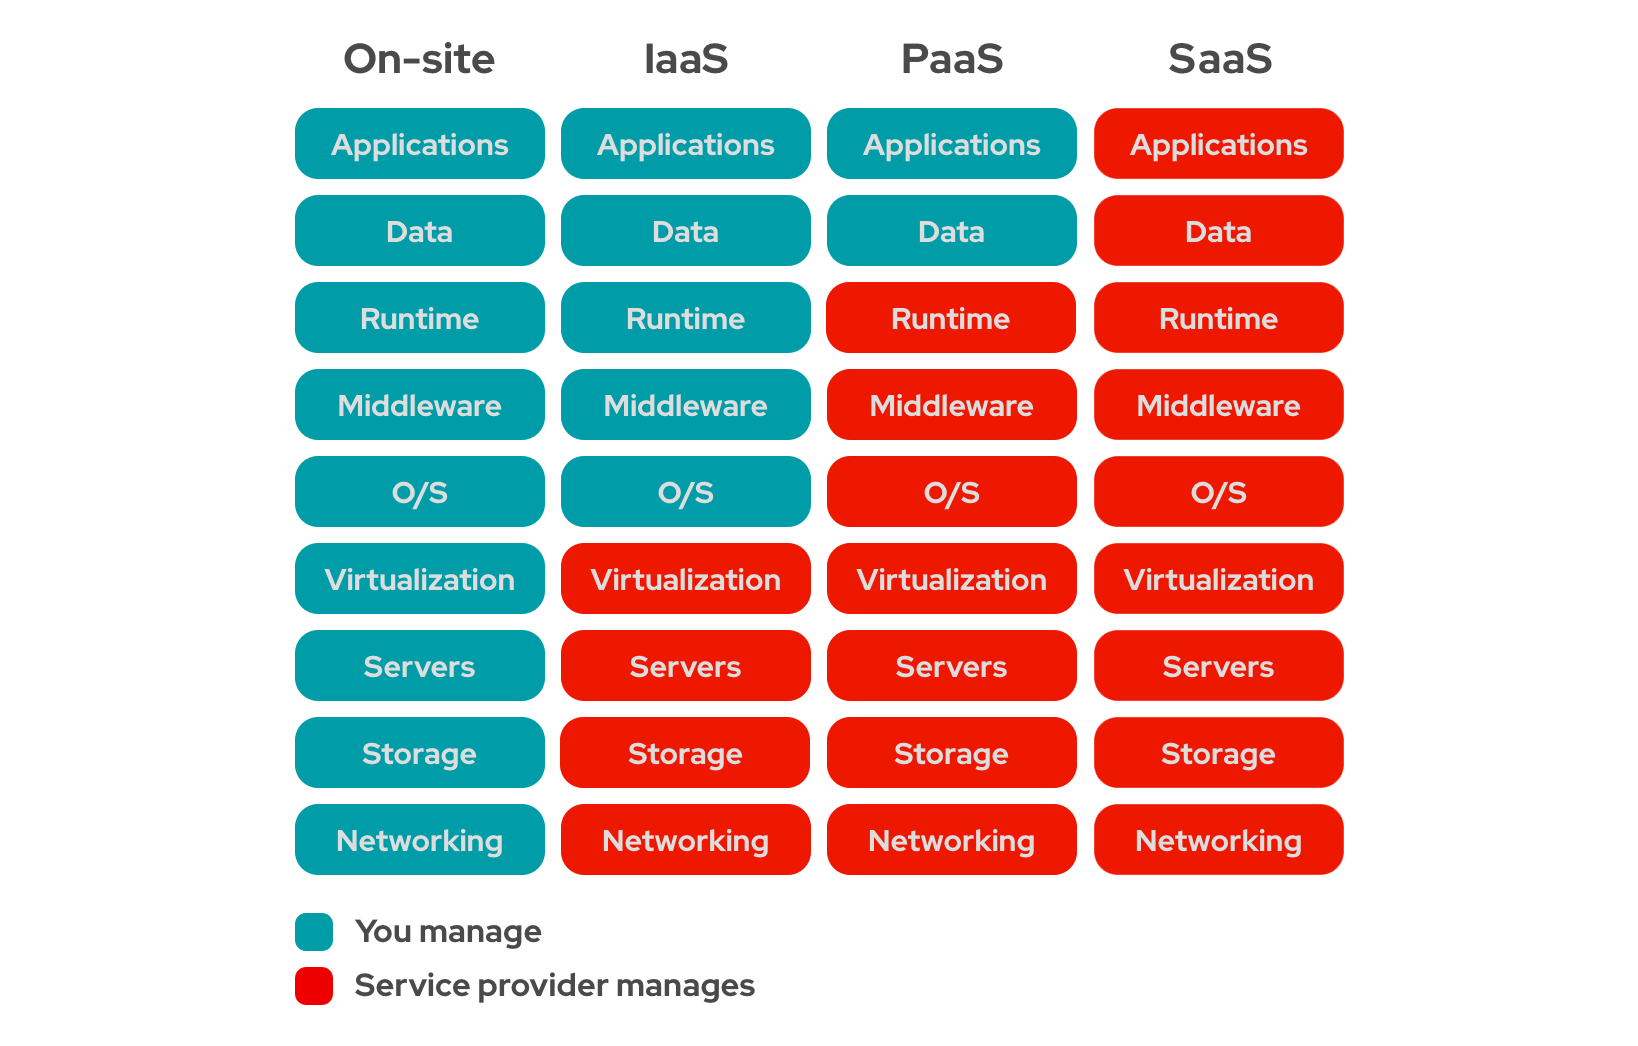
\includegraphics[width=\textwidth]{doc/logos/imgs/iaas-paas.png}
    \caption{ Distintos modelos de computación en la nube.
	\href{https://www.redhat.com/es/topics/cloud-computing/iaas-vs-paas-vs-saas}{RedHat -
	CC}}
    \label{fig:tipos-de-cc}
\end{figure}
\FloatBarrier

En el mercado existen distintas empresas que nos ofrecen este tipo de servicios, podemos
destacar: \href{https://aws.amazon.com/es/elasticbeanstalk/}{AWS Elastic Beanstalk},
\href{https://dashboard.heroku.com/login}{Heroku} o \href{https://vercel.com/}{Vercel}
entre otros.

Mientras que Vercel no soporta (por el momento) despliegues basados en imágenes de docker,
que es la \hyperref[sec:proceso-despliegue]{forma de despliegue que persigo}, y AWS
solicita información bancaria, he utilizado Heroku.

\section{Proceso de despliegue}
\label{sec:proceso-despliegue}
Para poder desplegar una aplicación en Heroku, es necesario acceder al panel de
administración y crearnos una "app". Sin embargo, existe un CLI \footnote{Interfaz de
línea de comandos} que se instala en nuestro sistema y nos permite realizar de forma más
cómoda las configuraciones necesarias.

A la hora de desplegar el código, Heroku nos ofrece distintas formas, una de ellas es
poner a la escucha una rama del repositorio de GitHub a cualquier tipo de cambio para
auto-desplegar. Sin embargo, este proyecto tiene muchos \textit{assets}, los ficheros con
los datos de las defunciones que no están versionados por el control de versiones. Este
motivo y el poco margen de personalización que provoca este método sobre con que
configuración queremos arrancar el servidor me hizo desestimar esta forma.

El método que he seguido ha sido crear un contenedor de la aplicación que luego publicamos
en la "app" creada en Heroku. Los contenedores nos permite tener una portabilidad absoluta
ya que podemos poner en marcha la aplicación en cualquier sistema operativo sin
preocuparnos de las dependencias necesarias.

El contenedor y su configuración se define como código en un archivo de texto plano
llamado \codeword{Dockerfile} en él se define el software necesario a instalar, las
dependencias del proyecto, se expone el host y el puerto como variables de entorno que
serán utilizadas por Heroku. También se especifica en el comando que ejecuta el contenedor
el número de procesos \footnote{la versión gratuita solo admite 2.} que va a ejecutar el
dyno. 

\FloatBarrier
\begin{figure}[h]
	\centering	
	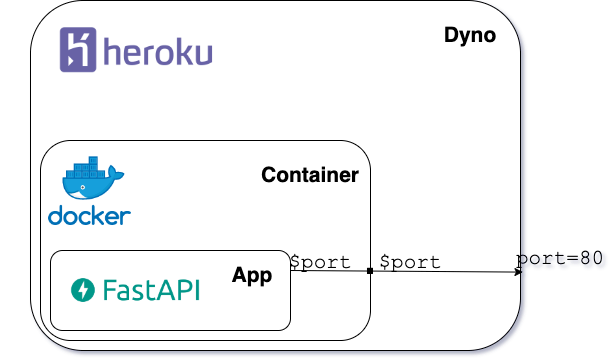
\includegraphics[width=\textwidth]{doc/logos/imgs/deployd.png}
	\caption{ Arquitectura del despliegue. }
    \label{fig:arq-deploy}
\end{figure}
\FloatBarrier

\begin{itemize}
    \item \textit{Dyno} es un contenedor liviano con Linux en los que Heroku ejecuta la
    aplicación.
\end{itemize}

Utilizando la CLI podemos ver el sistema de registros (que también está disponible en el
\textit{dashboard} web) con el que podemos monitorizar todas las peticiones que se
realizan así como los reinicios de la máquina virtual y el estado del servidor.

\FloatBarrier
\begin{figure}[h]
	\centering	
	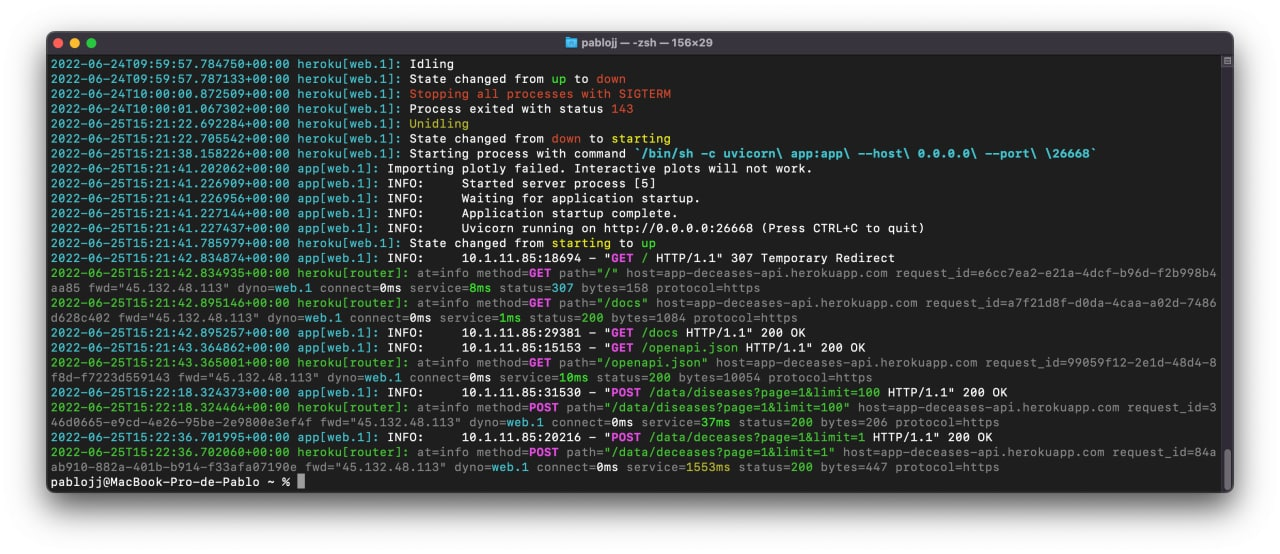
\includegraphics[width=\textwidth]{doc/logos/imgs/logs.jpg}
	\caption{ \textit{Logs} de la aplicación desplegada. }
    \label{fig:heroku-logs}
\end{figure}
\FloatBarrier

\section{Coste del despliegue}
\label{sec:despliegue}

Durante el proceso de desarrollo y las primeras pruebas se ha utilizado la modalidad "Free
\& Hobby" que nos permite desplegar la aplicación de forma gratuita con una seria
limitación: la máquina entra en estado de reposo tras 30 minutos de inactividad, lo que
hace que cuando se reciba cualquier petición haya que encender el contenedor, además el
número de procesos está limitado a 2 máquinas.

Para la puesta en producción debería de contratar la tarifa "Standard 1X" que nos ofrece
512MB de RAM, con ilimitado número de procesos, sin estado de procesos y nos incluye un
sistema de métricas y avisos que no está disponible en la versión gratuita.

\chapter{Conclusiones y trabajos futuros}
Al principio de este documento se definieron unos objetivos a alcanzar, vamos a analizar
en este capítulo si se han cumplido y cuales serian las lineas de trabajo futuras de
acuerdo con las necesidades expresadas por nuestros usuarios.

El principal reto que tenía que satisfacer este trabajo era la exposición de estos datos
de dominio público para que los usuarios diana fueran capaces de poder conocer la
evolución de las causas de muerte. Esto se ha conseguido implementando una serie de
interfaces agnósticas que permiten acceder al sistema desplegado y realizar consultas sin
necesidad de ningún tipo de configuración. 

Esto avanza en la necesidad de mejora que tiene el \Gls{SNS} para prevenir el máximo número
posible de muertes gracias a las aplicaciones integrales que pueden ser desarrolladas
utilizando este sistema.

Me siento orgulloso de haber sido capaz de realizar con éxito un proyecto de ingeniería de
software desde sus inicios, objetivos, planificación de recursos hasta estructurar una
metodología basada en desarrollo ágil que me ha permitido aportar valor inmediato en las
iteraciones y todo lo que he aprendido de ellos son cosas que pasan desapercibidas en otras situaciones.

\section{Trabajos futuros}
Voy a exponer la principal línea de trabajo por la que sería -bajo mi opinión- interesante seguir:
\begin{itemize}
    \item Permitir la integración de distintas fuentes de datos con otros modelos de datos
    también distintos. Por ejemplo, con otras escalas temporales.
\end{itemize}
Este proyecto es libre y está publicado con licencia \cite{gplv3} por lo que, en
correlación también con el desarrollo ágil, cualquier usuario puede abrir tareas y
proponer cambios.